%%%%%%%%%---Packages and document settings---%%%%%%%%%
\documentclass[twoside,twocolumn]{article}

  \usepackage{blindtext}      % Package to generate dummy text throughout this template 
  
  \usepackage[sc]{mathpazo}   % Use the Palatino font
  \linespread{1.05}           % Line spacing - Palatino needs more space between lines
  \usepackage[T1]{fontenc}    % Use 8-bit encoding that has 256 glyphs
  \usepackage{microtype}      % Slightly tweak font spacing for aesthetics
  
  \usepackage[spanish]{babel} % Language hyphenation and typographical rules
  
  \usepackage[hmarginratio=1:1,top=32mm,columnsep=20pt]{geometry}     % Document margins
  \usepackage[hang, small,labelfont=bf,up,textfont=it,up]{caption}    % Custom captions under/above floats in tables or figures
  \usepackage{booktabs}       % Horizontal rules in tables
  
  \usepackage{lettrine}       % The lettrine is the first enlarged letter at the beginning of the text
  
  \usepackage{enumitem}       % Customized lists
  \setlist[itemize]{noitemsep}  % Make itemize lists more compact
  
  \usepackage{abstract}       % Allows abstract customization
  \renewcommand{\abstractnamefont}{\normalfont\bfseries}      % Set the "Abstract" text to bold
  \renewcommand{\abstracttextfont}{\normalfont\small\itshape} % Set the abstract itself to small italic text
  
  \usepackage{titlesec}                                   % Allows customization of titles
  \renewcommand\thesection{\Roman{section}}               % Roman numerals for the sections
  \renewcommand\thesubsection{\roman{subsection}}         % roman numerals for subsections
  \renewcommand\thesubsubsection{\arabic{subsubsection}}   % roman numerals for subsections
  \titleformat{\section}[block]{\Large\scshape\centering}{\thesection.}{1em}{}    % Change the look of the section titles
  \titleformat{\subsection}[block]{\large}{\thesubsection.}{1em}{}                % Change the look of the section titles
  \titleformat{\subsubsection}[block]{\it}{\quad\footnotesize\thesubsubsection.}{0.5em}{}                % Change the look of the section titles
  
  \usepackage{fancyhdr}     % Headers and footers
  \pagestyle{fancy}         % All pages have headers and footers
  \fancyhead{}              % Blank out the default header
  %\fancyfoot{}              % Blank out the default footer
  \fancyhead[C]{Running title $\bullet$ May 2016 $\bullet$ Vol. XXI, No. 1}   % Custom header text
  %\fancyfoot[RO,LE]{\thepage} % Custom footer text
  
  \usepackage{titling}      % Customizing the title section
  
  \usepackage{hyperref}     % For hyperlinks in the PDF
  \usepackage{graphics}     % standard graphics specifications
  \usepackage{graphicx}     % alternative graphics specifications
  \usepackage{longtable}    % helps with long table options
  \usepackage{siunitx}      % para las unidades
  

%%%%%%%%%---Title, authors, date & abstract---%%%%%%%%%
\title{Implementación de una librería para la detección y el análisis de interacciones de partículas con CMOS}
  \author{%
    \textsc{Darío Federico Balmaceda} \\[1ex]     %  Your name
    \normalsize Laboratorio Detección de Partículas y Radiación. Centro Atómico Bariloche \\                                    %  Your institution
    \normalsize \href{mailto:leschatten@gmail.com}{\texttt{leschatten@gmail.com}}                   %  Your email address
    %\and                                                                      %  Uncomment if 2 authors are require
    %\textsc{Jane Smith} \\[1ex]                  % duplicate these 4 lines
    %\normalsize University of Utah \\ % Second author's institution           % if more
    %\normalsize \href{mailto:jane@smith.com}{jane@smith.com}
  }
  \date{\today}                                                                % Leave empty to omit a date
  \renewcommand{\maketitlehookd}{
    \begin{abstract}
      \noindent
      Lorem ipsum dolor sit amet, consectetuer adipiscing elit. Etiam lobortis facilisis sem. Nullam nec mi et
        nequepharetra sollicitudin. Praesent imperdiet mi nec ante. Donec ullamcorper, felis non sodales commodo,
        lectusvelit ultrices augue, a dignissim nibh lectus placerat pede. Vivamus nunc nunc, molestie ut, ultricies
        vel,semper in, velit. Ut porttitor. Praesent in sapien. Lorem ipsum dolor sit amet, consectetuer adipiscing
        elit.Duis fringilla tristique neque. Sed interdum libero ut metus. Pellentesque placerat. Nam rutrum augue
        aleo. Morbi sed elit sit amet ante lobortis sollicitudin. Praesent blandit blandit mauris. Praesent lectus
        tellus,aliquet aliquam, luctus a, egestas a, turpis. Mauris lacinia lorem sit amet ipsum. Nunc quis urna
        dictumturpis accumsan semper
      %TODO: ABSTRACT
    \end{abstract}
  }

  \setlength{\droptitle}{-4\baselineskip}                 % Move the title up
  \pretitle{\begin{center}\Large\bfseries}                 % Article title formatting
  \posttitle{\end{center}}                                % Article title closing formatting

%
  %%%%%%%%%%%%%%%%%%%%%%%%%%%%%%%%%%%%%%%%%%
  %%%%                                 %%%%%
  %%%%  And now, begin the document... %%%%%
  %%%%                                 %%%%%
  %%%%%%%%%%%%%%%%%%%%%%%%%%%%%%%%%%%%%%%%%%
\begin{document}
  
  \maketitle              % Print the title
  
  %%%%%%%%%%%%%%%%%%%%%%%%%%%%%%%%%%%%%%%%%%%%%%%%%%%
  \section{Introducción}
    %\cite{Lane}
    \lettrine[nindent=0em,lines=3]{L} orem ipsum dolor sit amet, consectetur adipiscing elit.
      Etiam lobortis facilisis sem. Nullam nec mi et nequepharetra sollicitudin.
      Praesent imperdiet mi nec ante. Donec ullamcorper, felis non sodales commodo,
      lectusvelit ultrices augue, a dignissim nibh lectus placerat pede.
    %TODO: reemplazar esto

    \subsection{Sensores CMOS-APS}
      Un sensor de píxeles activos (APS por sus siglas en inglés) es un sensor que detecta la radiación basado en tecnología CMOS.
      Este tipo de sensores son ampliamente utilizados de manera comercial debido a su
      bajo costo de producción y sus buenos resultados en fotografía.
      Estos sensores están presentes en teléfonos celulares, ordenadores portatiles, cámaras de acción,
      y en la mayoría de los dispositivos electrónicos que posee una cámara.

      Los sensores consisten en un arreglo matricial de fotodiodos, 
      que producen una corriente eléctrica que varía en función de la intensidad de luz recibida.
      Por cada fotodiodo, se incorpora un amplificador y un conversor analógico digital (ADC) para la lectura de los datos.
  

    \subsection{Interacción de la radiación de partículas con la materia}

    \subsection{Rayos cósmicos}
    
    \subsection{Picos $K_{\alpha}$ y $K_{\beta}$}

  %%%%%%%%%%%%%%%%%%%%%%%%%%%%%%%%%%%%%%%%%%%%%%%%%%%
  \section{Configuración experimental}

    \subsection{Raspberry}

    \subsection{Sensor CMOS}
      Se ha utilizado el sensor OmniVision OV5647 de la cámara Raspicam V1.3 cuyo precio ronda los 25 dólares.
      El sensor posee una resolución de	$2592$x$1944$ pixeles, lo que le una resolución total de $5$ MP.
      El tamaño de un píxel de \SI{1.4}{\micro\meter} x \SI{1.4}{\micro\meter}.
      El FULL-WELL-CAPACITY es de $4300$ electrones. %No sé como se traduce esto.
      El sensor posee un ADC de 10 bits por pixel.

      El sensor CMOS posee un filtro de Bayer, el mismo consiste en un arreglo de filtros rojos, verdes y azules
      dispuestos como se muestra en la Fig.~\ref{fig:bayer}. De esta forma, cada pixel posee la información de una longitud de onda,
      esto permite una composición de la imagen en 3 colores diferentes, de manera análoga al ojo humano.

      \begin{figure}[h]
        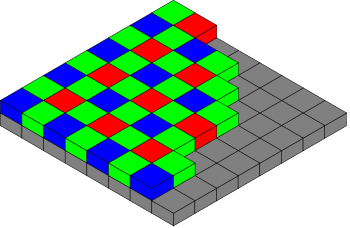
\includegraphics[width=0.35\textwidth]{figures/Bayer_pattern.png}
        \caption{Filtro de Bayer típico de un sensor CMOS-APS. Por cada 4 pixeles 2 son verdes, 1 es rojo y 1 es azul.
          El color verde es utilizado dos veces debido a la sensibilidad al verde del ojo humano.}
        \label{fig:bayer}
      \end{figure}

    \subsection{Librería raspiraw}
      Para la adquisicón de datos se utilizó la librería {\it raspiraw}\cite{raspiraw} debido a la rapidez con la que se toman los datos.
      En el apéndice~\ref{sec:ap_alternatives} se muestran otras alternativas que son más lentas para la toma de datos,
      pero que pueden resultar más simples y sencillas de implementar.

      %TODO:   Hablar sobre los parámetros que se le pueden variar

  %%%%%%%%%%%%%%%%%%%%%%%%%%%%%%%%%%%%%%%%%%%%%%%%%%% 
  \section{Resultados}
    Para probar el correcto funcionamiento de la librería, se utilizó el poder de procesamiento en dos aplicaciones diferentes.
    Una de ellas consistió en detectar Rayos Cósmicos, y la otra la de observar los picos $K_{\alpha}$ y $K_{\beta}$ de diferentes elementos.
    
    \subsection{Medición de Rayos Cósmicos}

    \subsection{Medición de picos $K_{\alpha}$ y $K_{\beta}$}

      \subsubsection{Cobre}

      \subsubsection{Aluminio}

      \subsubsection{Hierro}

      \subsubsection{Calcio}
    
  %%%%%%%%%%%%%%%%%%%%%%%%%%%%%%%%%%%%%%%%%%%%%%%%%%%
  \section{Conclusiones}
  %%%%%%%%%%%%%%%%%%%%%%%%%%%%%%%%%%%%%%%%%%%%%%%%%%%
  \section{Referencias}\label{}
    
    \bibliographystyle{siam}
    \bibliography{bibliography}

  %%%%%%%%%%%%%%%%%%%%%%%%%%%%%%%%%%%%%%%%%%%%%%%%%%%
  \section*{Agradecimientos}
    Se agradece la colaboración de Xavier Bertou por la experiencia brindada y por
    acompañar el trabajo en forma constante.

    A Miguel Sofo por la disponibilidad y por su flexibilidad a la hora de trabajar.
    % TODO: decidir, más gente? 
    % A Geraldina Gulop, Florencia  ¿?
   
  %%%%%%%%%%%%%%%%%%%%%%%%%%%%%%%%%%%%%%%%%%%%%%%%%%%
  \clearpage
  \appendix
  \section{Alternativas a Raspiraw}\label{sec:ap_alternatives}
  
  \section{Documentación de la librería}\label{sec:ap_doc}

    \subsection{rawImages}\label{sec:ap_doc:rawImages}

    \subsection{rawEvent}\label{sec:ap_doc:rawEvent}

    \subsection{rawFilters}\label{sec:ap_doc:rawFilters}

      En este header se incluyen filtros típicos utilizados para el procesamiento de imágenes \emph{rawPhoto\_t}.
      Estas son externas a la clase \emph{rawPhoto\_t}, por lo que deben ser pasadas como parámetros. 

\end{document}

    



